\documentclass[12pt,a4paper]{article}
\usepackage{graphicx}
\usepackage{amsmath}
\setlength{\topmargin}{0cm}
\input acentos
\input psfig.sty

% Create friendly environments for theorems, propositions, &c.
\newtheorem{theorem}{Theorem}[section]
\newtheorem{lemma}[theorem]{Lemma}
\newtheorem{proposition}[theorem]{Proposition}
\newtheorem{corollary}[theorem]{Corollary}
\newenvironment{proof}[1][Proof]{\begin{trivlist}
	\item[\hskip \labelsep {\bfseries #1}]}{\end{trivlist}}
\newenvironment{definition}[1][Definition]{\begin{trivlist}
	\item[\hskip \labelsep {\bfseries #1}]}{\end{trivlist}}
\newenvironment{example}[1][Example]{\begin{trivlist}
	\item[\hskip \labelsep {\bfseries #1}]}{\end{trivlist}}
\newenvironment{remark}[1][Remark]{\begin{trivlist}
	\item[\hskip \labelsep {\bfseries #1}]}{\end{trivlist}}
\newcommand{\bu}[1]{\mbox{$\mathbf{#1}$}}

\begin{document}

\begin{center}
  {\Large Uses and caveats of Latin Hypecube Sampling in the parameter space exploration of ecological models}

\begin{table}[hbt]{\small
\begin{tabular}{ll}
Authors        & Andre Chalom \\
               & Paulo Inacio Prado \\
Date           & 03/16/2012 \\
Affiliation    & Department of Ecology, \\
	       & University of Sao Paulo 
\end{tabular} }
\end{table}
\end{center}

\mbox{}\vspace{-14mm}\mbox{}


\section*{Abstract}
In recent years, both the scientific community and policy makers are gaining confidence in the formulation 
and use of mathematical models in ecological studies. We are thus seeing a flourishing of more elaborate
and complex models, and the questions related to the efficient, systematic and error-proof exploration of 
parameter spaces are of great importance to better understand, estimate confidences and make use of the output
from these models. In this work, we investigate some of the relevant questions related to parameter space
exploration, in particular using the technique known as Latin Hypercube Sampling, and assess how are these
questions being currently addressed in the literature.

\section{Introduction}\label{Introduction}
\subsection{Parameter spaces}
In order to better pose our questions, we need first to have a precise definition of what is the parameter space
of our models, and to distinguish the general use of this expression by the statistical and the modeling community.
** ROSS, 1990 **

Also, it should be mentioned that the parameter space may be constrained (for example, $a_1 + a_2 < 90$ degress) or unconstrained.

\dots

\subsection{Problems in PS exploration}
Next, we turn our attention to the kind of problems we might want to address with the exploration of the parameter space.
First, the simplest case is asking ``is there a region of my parameter space where condition X holds?'' This condition
might be, for example, the extinction or coexistance of species, some pattern of distribution or abundance of species.
We also might be interested in mapping where are these regions. In complex models, where several different regions might
exist where the qualitative results of the models are very different, we may ask how many of these regions are there, as well
as map the frontiers between them. 

Another class of problems arises when the model produces some quantitative response, and we are interessed in determining
the dependency of this response to the input parameters. For example, in models where limit cycles arise, we would like to know
how the period of the limit cycle varies with each of the parameters. Along with these questions, it may be extremely important
to assess the sensitivity of the model to small fluctuations in the parameters.
** KUEHN 2010 **
** HELTON 2003 **

All these problems may be formulated in a general way, defining some response from the model $\bu{Y}$ as a function of the
parameter vector $\bu{x}$:

\begin{equation}
	\bu{Y} = \bu{f}(\bu{x})
	\label{genmodel}
\end{equation}

In the equation \ref{genmodel}, all the quantities are vectors, indicated by the boldface. Here, 
$\bu{x} = [ x_1,x_2,\dots,x_n ]$ represent the parameters to the model $\bu{f}$, and $\bu{Y} = [ y_1,y_2,\dots,y_n ]$ 
represent the some quantitative response from the model.

\dots

\subsection{Stochastic models}
When dealing with stochastic models, like several relevant individual based models (IBM), the questions presented become
complicated by the fact that running the same model with exactly the same parameters might wield largely different results,
both quantitative and qualitatively. In this scenario,
\begin{itemize}
	\item Is is possible to formulate the stochastic and deterministic problems in a general way?
	\item What are the conditions for a stochastic model to be subject to parameter space exploration?
	\item Are there techniques that can be applied to the stochastic models to make them more amenable to PS exploration?
\end{itemize}

We also give an overview of Marko Chain Monte Carlo methods, and their relation with LHS.

\dots

\section{Latin Hypercube Sampling}
\subsection{Definition and use}
In this section, we describe the Latin Hypercube Sampling, and show how it can be used to efficiently solve the questions
posed in section \ref{Introduction}. We briefly compare it to some other techniques, like random sampling. We also discuss
what are the available implementations of LHS. 

Firstly, let us define, in the context of statistical sampling, what is a Latin Square:
\begin{definition}
If we divide each side in a square in $M$ intervals, and then take samples from the square, the resulting square will be called
Latin if and only if there is exactly one sample in each row and each column.
\end{definition}

From this definition, it is clear that the number of samples is fixed as $M$. It should be noted that, in the mathematical
literature, it is usual to refer to a somewhat different object as a Latin Square: this would be a square whose sides are 
divided in $M$ intervals, and is filled with $M$ different symbols, such that for each row and column there is exactly one 
occurrence of each symbol. The figure \ref{fig:glassLS} shows an example of one ``full'' Latin Square. If we restrict our
attention to just one color, we can visualize a Latin Square in the statistical sense.

\begin{figure}[htpb]
	\begin{center}
		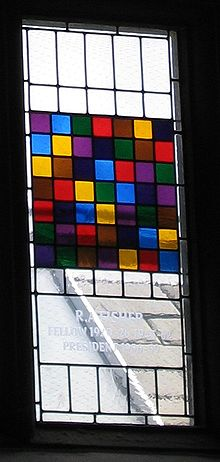
\includegraphics{glassLS.png}
	\end{center}
	\caption{A stained glass window at the Caius College, Cambridge, showing a full Latin Square. Notice how there is only one occurence of each color in each row and in each column.}
	\label{fig:glassLS}
\end{figure}

A Latin Hypercube is the generalization of the Latin Square to an arbitrary number of dimensions $n$. 

The first step to construct the Latin Hypercube is to divide each parameter dimension in M equally probable intervals. Thus, it
is necessary to assign some probability function to each parameter dimension. We will briefly discuss how this choice must
be made and how it might affect the result of the sampling.

\dots

\subsection{Algorithms and extensions}
As described above, the LH sampling generates an uniform distribution of samples in each parametric dimension. However, 
there is no guarantee that the correlation between two or more parameters will be zero, and the classical algorithm
from McKay \cite{McKay} usually produces correlations as high as 0.3 between pairs of factors, which can difficult or even
compromise further analyses. In this section, we will present and compare some algorithms designed to minimize pairwise 
as well as higher order correlations, or even to produce samples with zero correlation terms.

** YE **
** STEINBERG **


\dots

\subsection{Adaptative refinement}
Is it possible to adaptatively refine the grid in order to increase the number of points sampled, or if we decide to run
the analysis with double the points I have to start from scratch?

\dots

\subsection{Use of Latin Hypercube in ecological studies}
Here we present some relevant papers in the ecological literature that made use of LH sampling or similar parameter space
exploration techniques. We also try to summarize what are the prerequites that a model must fulfill in order to use it, 
what are the cautions that must be taken in running the sampling, what are the potential pitfalls interpreting the results.

\dots

\section{Making use of the results}
After applying the Latin Hypercube Sampling to an ecological model and gathering the results, what are the next steps? Here, we 
highlight some statistical analysis (like ANOVA) and numerical interpolation methods that can be used to make sense of the model
output.

\bibliography{chalom}

\end{document}
